\documentclass{urdpl}     % praca w języku polskim

% Lista wszystkich języków stanowiących języki pozycji bibliograficznych użytych w pracy.
% (Zgodnie z zasadami tworzenia bibliografii każda pozycja powinna zostać utworzona zgodnie z zasadami języka, w którym dana publikacja została napisana.)
\usepackage[english,polish]{babel}

% Użyj polskiego łamania wyrazów (zamiast domyślnego angielskiego).
\usepackage{polski}

\usepackage[utf8]{inputenc}

% dodatkowe pakiety

\usepackage{mathtools}
\usepackage{amsfonts}
\usepackage{amsmath}
\usepackage{amsthm}
\usepackage[hidelinks]{hyperref}
\usepackage{float}
\usepackage{listings}
\usepackage{graphicx}
\usepackage{subcaption}
\usepackage{booktabs} % Dla \toprule, \midrule, \bottomrule
\usepackage{multirow} 
\usepackage{tabularx} 
\usepackage{amssymb} 
\usepackage{listings}
\usepackage{xcolor}
\usepackage{array}
\usepackage{makecell}
\usepackage[flushleft]{threeparttable}
\usepackage[normalem]{ulem}
\usepackage{lineno}
\usepackage{makecell} %
\usepackage{csquotes}
\usepackage{courier}

% ------------------------
% --- < listingi > ---

\usepackage{listings}
\lstloadlanguages{TeX}
\renewcommand{\lstlistlistingname}{Spis listingów}
\renewcommand{\lstlistingname}{Listing}

\lstset{
	literate={ą}{{\k{a}}}1
           {ć}{{\'c}}1
           {ę}{{\k{e}}}1
           {ó}{{\'o}}1
           {ń}{{\'n}}1
           {ł}{{\l{}}}1
           {ś}{{\'s}}1
           {ź}{{\'z}}1
           {ż}{{\.z}}1
           {Ą}{{\k{A}}}1
           {Ć}{{\'C}}1
           {Ę}{{\k{E}}}1
           {Ó}{{\'O}}1
           {Ń}{{\'N}}1
           {Ł}{{\L{}}}1
           {Ś}{{\'S}}1
           {Ź}{{\'Z}}1
           {Ż}{{\.Z}}1,
	basicstyle=\footnotesize\ttfamily,
}

% defninicja stylu python
\lstdefinestyle{stylePython}{
    language=Python,
    commentstyle=\color{green},          % Kolor komentarzy
    keywordstyle=\color{blue},           % Kolor słów kluczowych
    numberstyle=\tiny\color{gray},       % Kolor i styl numerów linii
    stringstyle=\color{red},             % Kolor ciągów znaków
    basicstyle=\ttfamily\footnotesize,   % Podstawowy styl kodu
    breakatwhitespace=false,             % Automatyczne dzielenie wierszy
    breaklines=true,                     % Dzielenie długich linii
    keepspaces=true,                     % Zachowanie spacji
    numbers=left,                        % Numery linii po lewej
    numbersep=5pt,                       % Odstęp numerów od kodu
    showspaces=false,                    % Nie pokazuj spacji
    showstringspaces=false,              % Nie pokazuj spacji w ciągach znaków
    showtabs=false,                      % Nie pokazuj tabulacji
    tabsize=2                            % Rozmiar tabulacji
}

% defnicja stylu JAVA
\lstdefinestyle{javaStyle}{
    language=Java,
    basicstyle=\ttfamily\footnotesize,
    keywordstyle=\color{blue},
    commentstyle=\color{green!50!black}\itshape,
    stringstyle=\color{green},
    numberstyle=\tiny\color{gray},
    numbers=left,
    numbersep=5pt,                       % Odstęp numerów od kodu
    stepnumber=1,
    showspaces=false,                    % Nie pokazuj spacji
    tabsize=2,
    showstringspaces=false,
    breaklines=true,
    breakatwhitespace=false,             % Automatyczne dzielenie wierszy
    showtabs=false,                      % Nie pokazuj tabulacji
    keepspaces=true                    % Zachowanie spacji
}

\definecolor{stringcolor}{RGB}{163,21,21}    % pomarańczowy - stringi
\definecolor{typecolor}{RGB}{43, 145, 176}     % ciemny fiolet - klasy, typy

\lstdefinestyle{csStyle}{
    language=[Sharp]C, % dla C#; można zmienić na Java
    basicstyle=\ttfamily\footnotesize,
    keywordstyle=\color{blue},
    stringstyle=\color{stringcolor},
    commentstyle=\color{green!50!black}\itshape,
    morekeywords={class, public, private, protected, static, void, string, int, new}, % dodatkowe słowa kluczowe
    emphstyle=\color{typecolor}\bfseries, % klasy na fioletowo
    numbers=left,
    numbersep=5pt,                       % Odstęp numerów od kodu
    numberstyle=\tiny\color{gray},
    stepnumber=1,
    breaklines=true,
    showspaces=false,                    % Nie pokazuj spacji
    tabsize=2,
    showstringspaces=false,
    breakatwhitespace=false,             % Automatyczne dzielenie wierszy
    showtabs=false,                      % Nie pokazuj tabulacji
    keepspaces=true                    % Zachowanie spacji  
}

\lstdefinestyle{matlabStyle}{
    language=Matlab,
    basicstyle=\ttfamily\footnotesize,  % Mała czcionka monospaced
    keywordstyle=\color{blue}\bfseries, % Słowa kluczowe na niebiesko i pogrubione
    stringstyle=\color{red},            % Ciągi znaków na czerwono
    commentstyle=\color{green!50!black}\itshape, % Komentarze na zielono, kursywa
    morekeywords={figure, imread, imshow, title, imhist, histeq, graythresh, imbinarize, stretchlim, imadjust}, % Dodatkowe słowa kluczowe MATLAB
    numbers=left,                        % Numeracja linii po lewej
    numbersep=5pt,                       % Odstęp numerów od kodu
    numberstyle=\tiny\color{gray},       % Mała, szara czcionka numerów linii
    stepnumber=1,                         % Numeracja co 1 linię
    breaklines=true,                      % Łamanie długich linii
    showspaces=false,                     % Nie pokazuj spacji
    showstringspaces=false,               % Nie pokazuj spacji w stringach
    showtabs=false,                        % Nie pokazuj tabulatorów
    tabsize=4,                             % Tabulacja 4 spacje
    breakatwhitespace=false,               % Automatyczne łamanie wierszy
    keepspaces=true                        % Zachowanie spacji  
}

\definecolor{lightgray}{rgb}{0.9,0.9,0.9}
    % \definecolor{blue}{rgb}{0,0,1}
    \definecolor{green}{rgb}{0,0.6,0}
    % \definecolor{red}{rgb}{0.6,0,0}
    \definecolor{gray}{rgb}{0.5,0.5,0.5}

% % ------------------------
\AtBeginDocument{
	\renewcommand{\tablename}{Tabela}
	\renewcommand{\figurename}{Rys.}   
    \newcommand{\listingname}{Listing}
}

% ------------------------
% --- < tabele > ---

% defines the X column to use m (\parbox[c]) instead of p (`parbox[t]`)
\newcolumntype{C}[1]{>{\hsize=#1\hsize\centering\arraybackslash}X}


%---------------------------------------------------------------------------

\author{Oleksii Nawrocki, Tomasz Nowak}
\shortauthor{O. Nawrocki, T. Nowak}
\noAlbum{oa131400, tn131478}

\titlePL{Projekt - BiometricSafe}
\titleEN{Project - BiometricSafe \LaTeX}

\shorttitlePL{Projekt - BiometricSafe} % skrócona wersja tytułu jeśli jest bardzo długi
\shorttitleEN{Project - BiometricSafe \LaTeX}

\thesistype{Sprawozdania\\ Grupa: 02 }

\thesisDone{Prowadzący}
\supervisor{dr Zbigniew Gomółka}
%\supervisor{Jan Nowak PhD}

\degreeprogramme{Informatyka}
%\degreeprogramme{Computer Science}

\date{2025}

\department{Instytut Informatyki}
%\department{Institute of Computer Science}

\faculty{Wydział Nauk Ścisłych i Technicznych}
%\faculty{Faculty of Science and Technology}



\setlength{\cftsecnumwidth}{10mm}

%---------------------------------------------------------------------------
\setcounter{secnumdepth}{4}
\brokenpenalty=10000\relax

% --------------------------------------------------------------------------
% główna część pracy
% --------------------------------------------------------------------------

\begin{document}

\titlepages

\chapter{Dokumentacja}

\section*{Streszczenie}
Niniejszy dokument opisuje aplikację desktopową stworzoną w języku Python z użyciem biblioteki Tkinter, której celem jest zabezpieczanie plików za pomocą unikalnych cech biometrycznych – odcisku palca użytkownika. System wykorzystuje ekstrakcję punktów charakterystycznych (minucji) i przekształca je na klucz kryptograficzny, umożliwiając szyfrowanie i deszyfrowanie plików.

\section{Technologie i biblioteki}
Projekt został zaimplementowany z użyciem następujących technologii i bibliotek:
\begin{itemize}
	\item \textbf{Python 3.x}
	\item \textbf{Tkinter} – GUI (graficzny interfejs użytkownika)
	\item \textbf{OpenCV} – przetwarzanie obrazu
	\item \textbf{scikit-image} – szkieletowanie obrazu (skeletonization)
	\item \textbf{cryptography (Fernet)} – symetryczne szyfrowanie danych
	\item \textbf{NumPy} – obliczenia numeryczne
	\item \textbf{PIL (Pillow)} – manipulacja obrazami w GUI
\end{itemize}

\section{Opis działania}

\subsection{1. Przetwarzanie obrazu odcisku palca}
Obraz wejściowy zostaje przekształcony do skali szarości i przefiltrowany przy użyciu filtra Gaussa. Następnie obraz zostaje zbinarnizowany metodą Otsu i poddany procesowi \textit{skeletonization}, by uprościć strukturę odcisku.

\subsection{2. Ekstrakcja punktów minucji}
Minucje to punkty charakterystyczne, takie jak zakończenia linii lub bifurkacje. System analizuje sąsiedztwo każdego punktu szkieletu, aby znaleźć potencjalne minucje.

\subsection{3. Generowanie klucza szyfrującego}
Zestaw punktów minucji jest konwertowany na łańcuch tekstowy i haszowany przy użyciu SHA-256. Na podstawie tego hasza tworzony jest klucz szyfrujący (Fernet), który jest następnie używany do szyfrowania lub odszyfrowywania pliku.

\subsection{4. Porównanie odcisków palców}
Podczas deszyfrowania system porównuje odcisk referencyjny (z użycia przy szyfrowaniu) z nowym odciskiem dostarczonym przez użytkownika. Miara podobieństwa jest oparta na średniej odległości euklidesowej między punktami.

\section{Interfejs użytkownika}

Poniżej przedstawiono główne etapy działania aplikacji w formie zrzutów ekranu:

\begin{figure}[H]
	\centering
	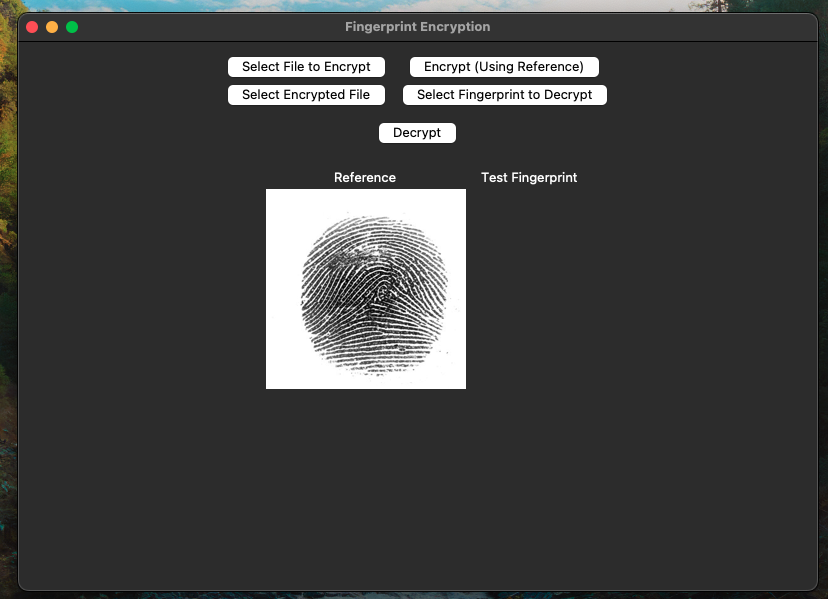
\includegraphics[width=\linewidth]{docs/app.png}
	\caption*{Widok głównego okna aplikacji}
\end{figure}

\begin{figure}[H]
	\centering
	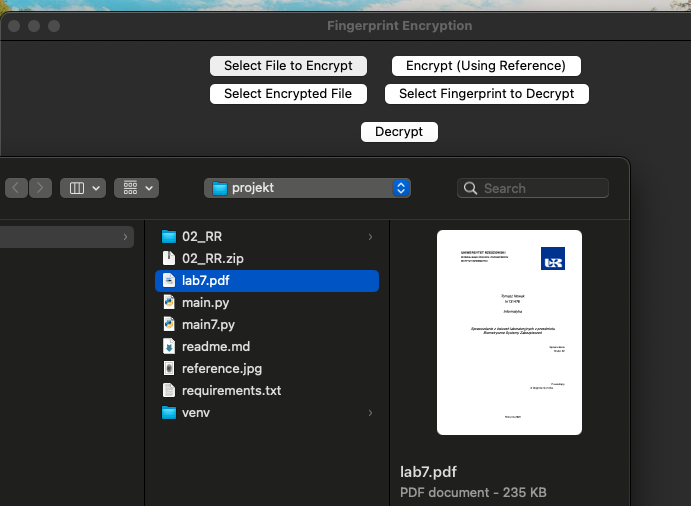
\includegraphics[width=0.85\linewidth]{docs/selectFileToEncrypt.png}
	\caption*{Wybór pliku do zaszyfrowania}
\end{figure}

\begin{figure}[H]
	\centering
	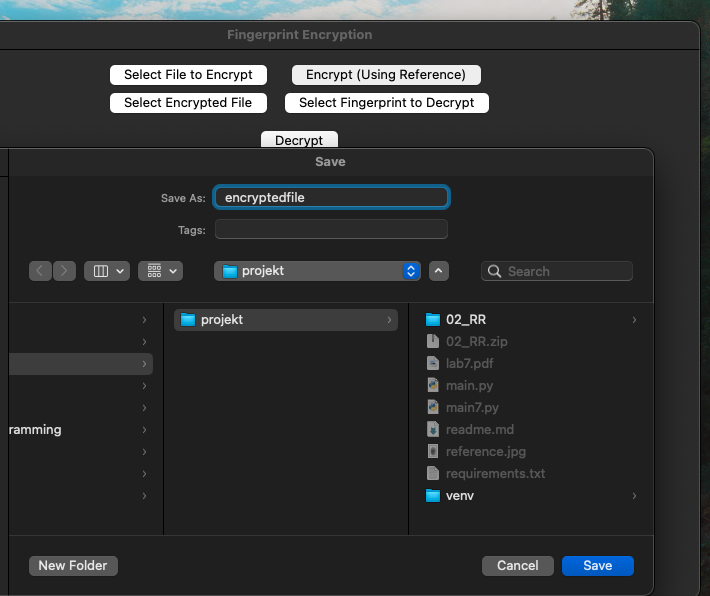
\includegraphics[width=0.85\linewidth]{docs/saveEncryptedFile.png}
	\caption*{Zapis zaszyfrowanego pliku}
\end{figure}

\begin{figure}[H]
	\centering
	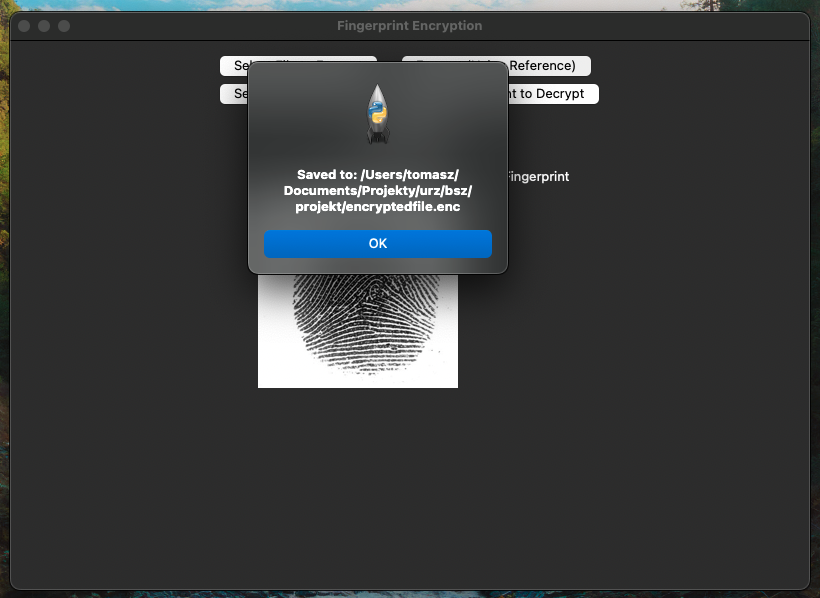
\includegraphics[width=0.85\linewidth]{docs/savedEncryptedFile.png}
	\caption*{Potwierdzenie zapisu zaszyfrowanego pliku}
\end{figure}

\begin{figure}[H]
	\centering
	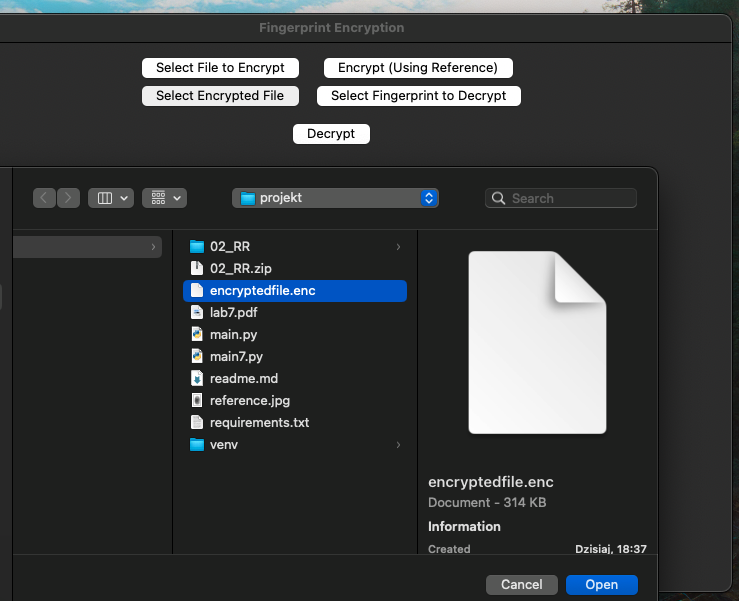
\includegraphics[width=0.85\linewidth]{docs/selectEncryptedFile.png}
	\caption*{Wybór pliku zaszyfrowanego do deszyfrowania}
\end{figure}

\begin{figure}[H]
	\centering
	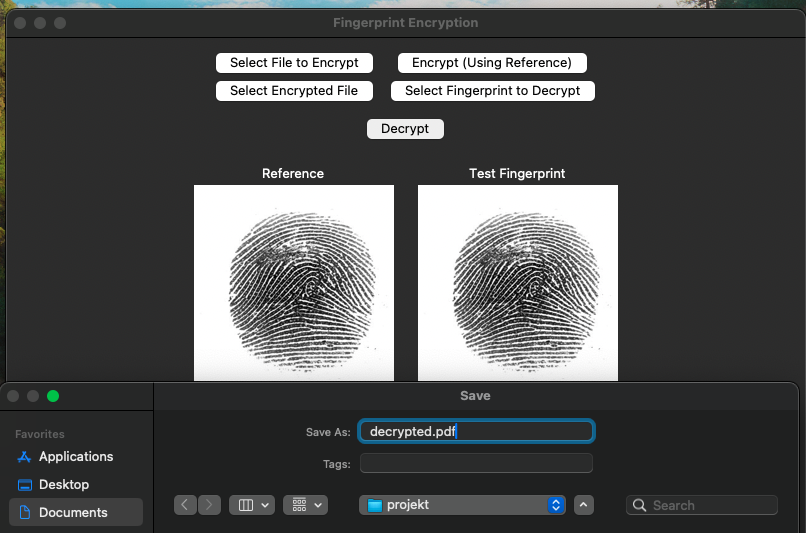
\includegraphics[width=0.49\linewidth]{docs/DecryptedViaValidFingerprint.png}
	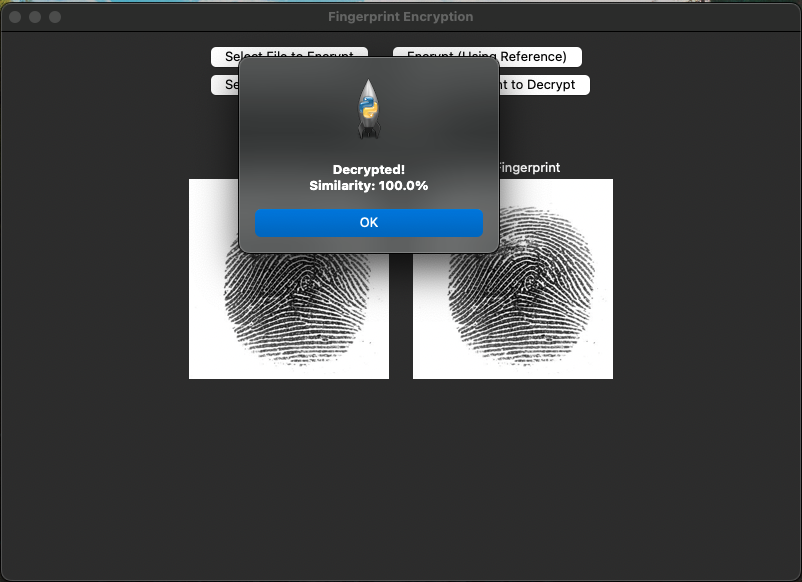
\includegraphics[width=0.49\linewidth]{docs/decryptedFileNotify.png}
	
	\vspace{0.5em}
	
	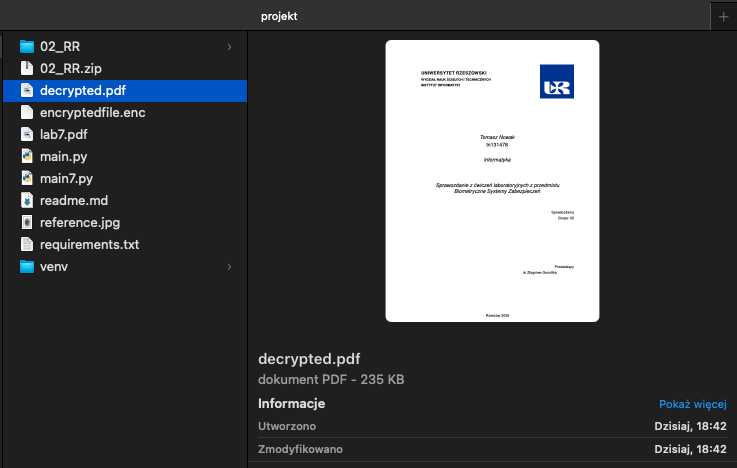
\includegraphics[width=0.85\linewidth]{docs/decryptedFile.png}
	\caption*{Deszyfrowanie z poprawnym odciskiem palca}
\end{figure}

\begin{figure}[H]
	\centering
	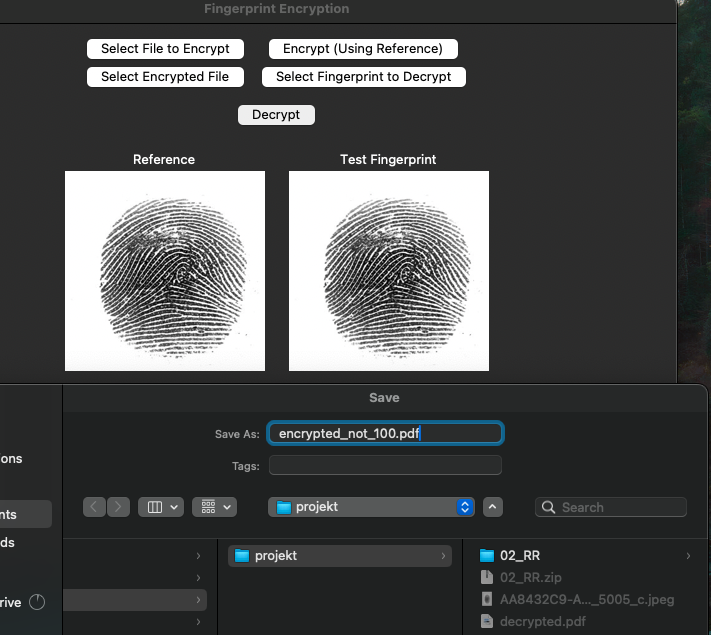
\includegraphics[width=0.49\linewidth]{docs/decryptedWithChangedValidImage.png}
	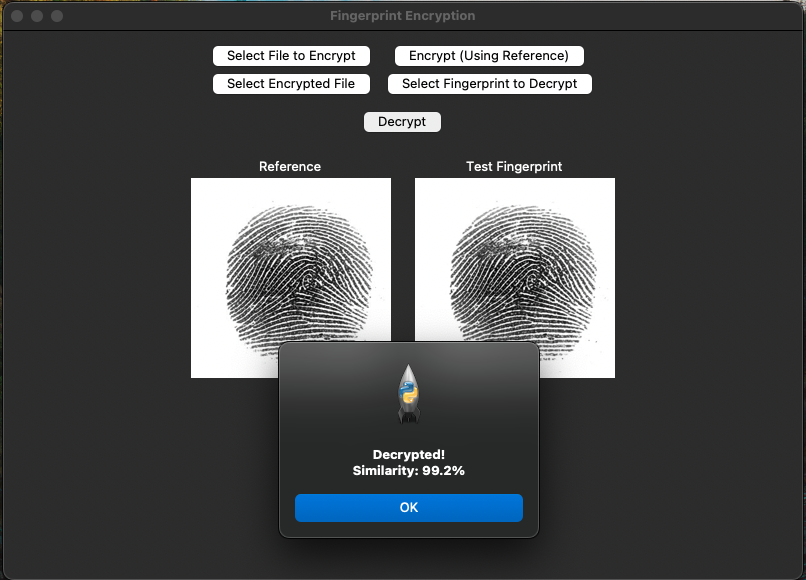
\includegraphics[width=0.49\linewidth]{docs/decryptedWithChangedValidImageNotify.png}
	
	\vspace{0.5em}
	
	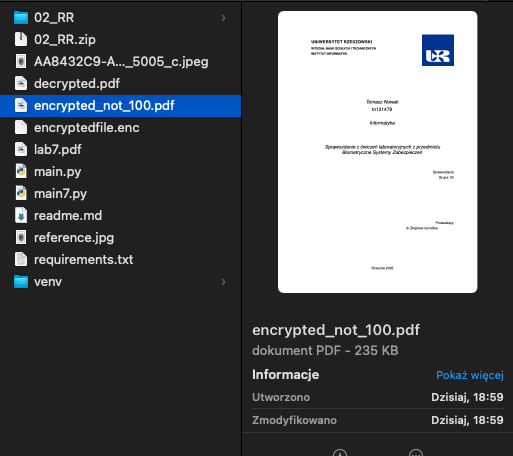
\includegraphics[width=0.85\linewidth]{docs/decryptedWithChangedValidImageFile.png}
	\caption*{Deszyfrowanie z lekko zmienionym, ale poprawnym obrazem}
\end{figure}

\begin{figure}[H]
	\centering
	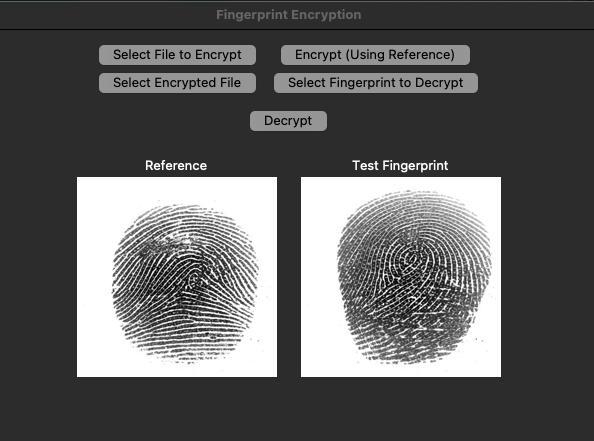
\includegraphics[width=0.49\linewidth]{docs/decryptViaInvalidFingerprint.png}
	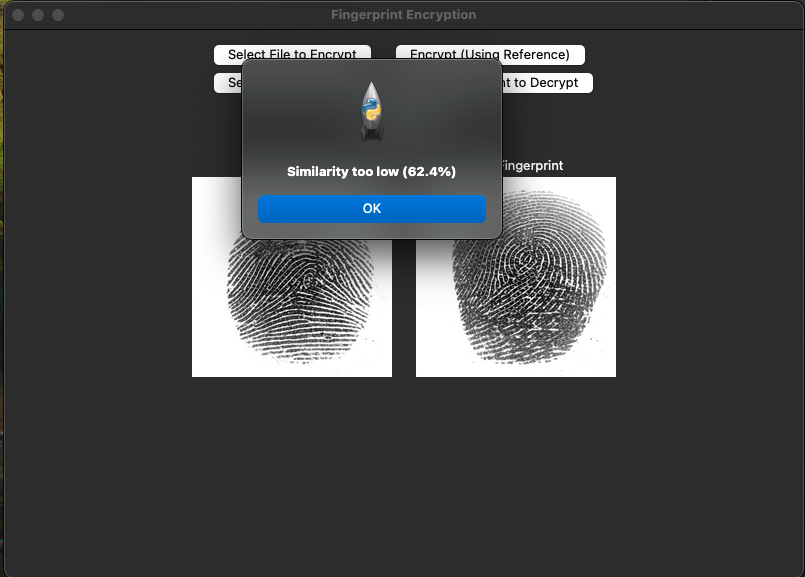
\includegraphics[width=0.49\linewidth]{docs/decryptViaInvalidFingerprintNotify.png}
	\caption*{Próba deszyfrowania z błędnym odciskiem palca}
\end{figure}

\section{Instrukcja obsługi}

\begin{enumerate}
	\item Uruchom aplikację.
	\item Kliknij „Wybierz plik do zaszyfrowania” i wybierz plik.
	\item Kliknij „Szyfruj (używając referencji)” – zostanie użyty obraz \texttt{reference.jpg}.
	\item Aby odszyfrować, wybierz zaszyfrowany plik oraz nowy obraz odcisku palca.
	\item Kliknij „Deszyfruj”. Jeśli odcisk jest zgodny, plik zostanie odszyfrowany.
\end{enumerate}

\section{Bezpieczeństwo}

Bezpieczeństwo aplikacji bazuje na dwóch poziomach:
\begin{itemize}
	\item Unikalność klucza – generowany z danych biometrycznych.
	\item Szyfrowanie symetryczne – za pomocą Fernet (AES w trybie CBC z HMAC).
\end{itemize}

\section{Zastosowania}
\begin{itemize}
	\item Bezpieczne przechowywanie danych lokalnych.
	\item Systemy kontroli dostępu.
	\item Przykład zastosowania biometrii w kryptografii.
\end{itemize}

\section*{Podsumowanie}
Aplikacja stanowi prosty, ale skuteczny przykład integracji biometrii i kryptografii w celu ochrony danych. Poprzez użycie cech odcisków palców jako źródła kluczy szyfrujących, system zapewnia wysoki poziom personalizacji i bezpieczeństwa.

\end{document}
